% !TEX encoding = UTF-8 Unicode
% Vorlage für eine Bachelorarbeit
% Siehe auch LaTeX-Kurs von Mathematik-Online
% www.mathematik-online.org/kurse
% Anpassungen für die Fakultät für Mathematik
% am KIT durch Klaus SpitzmÃŒller und Roland Schnaubelt Dezember 2011

\documentclass[12pt,a4paper]{scrartcl}
% scrartcl ist eine abgeleitete Artikel-Klasse im Koma-Skript
% zur Kontrolle des Umbruchs Klassenoption draft verwenden


% die folgenden Packete erlauben den Gebrauch von Umlauten und ß
% in der Latex Datei
\usepackage[utf8]{inputenc}
% \usepackage[latin1]{inputenc} %  Alternativ unter Windows
\usepackage[T1]{fontenc}
\usepackage[ngerman]{babel}


\usepackage[pdftex]{graphicx}
\usepackage{latexsym}
\usepackage{amsmath,amssymb,amsthm}

% Links einbinden:
\usepackage[colorlinks=true,urlcolor=blue,citecolor=blue,linkcolor=blue]{hyperref}

% SI-Units einbinden:
\usepackage{siunitx}
\sisetup{locale = DE ,per-mode = symbol}

% Abstand obere Blattkante zur Kopfzeile ist 2.54cm - 15mm
\setlength{\topmargin}{-15mm}


\begin{document}
  % Keine Seitenzahlen im Vorspann
  \pagestyle{empty}

  % Titelblatt der Arbeit
  \begin{titlepage}

    
\includegraphics[scale=0.45]{kit-logo.jpg} 
    \vspace*{2cm} 

 \begin{center} \large 
    
    Seminararbeit
    \vspace*{2cm}

    {\huge Stauindex}
    \vspace*{2.5cm}

    Markus Scherer\\
    Christof Urbaczek\\
    Nils Hennemann
    
    \vspace*{1.5cm}

    Datum der Abgabe
    \vspace*{3.5cm}

    Betreuung: Dr.-Ing. Bastian Chlond \\[1cm]
    Fakultät für Bauingenieurwesen \\[0.5cm]
    Institut für Verkehrswesen \\[1cm]
    
		Karlsruher Institut für Technologie
  \end{center}
\end{titlepage}



  % Inhaltsverzeichnis
  \tableofcontents

\newpage
 


  % Ab sofort Seitenzahlen in der Kopfzeile anzeigen
  \pagestyle{headings}
  
%%%%%%%%%
% 1) Einleitung %
%%%%%%%%%
\section{Einleitung}




%%%%%%%%%%%%%%%%
% 2) Technische Umsetzung  %
%%%%%%%%%%%%%%%%
\newpage  
\section{Technische Umsetzung}


%%%%%%%%%%%%%
% 3) Datenauswertung  %
%%%%%%%%%%%%%
\newpage
\section{Datenauswertung}

Im folgenden Kapitel soll das entwickelte Verfahren Anwendung bei der Verkehrsanalyse verschiedener Städte finden. Zunächst wird eine Plausibilisierung der aus google maps extrahierten Daten durchgeführt, indem diese mit gesicherten amtlichen Daten verglichen werden. 
Im Anschluss daran werden die aus bing maps gewonnenen Verkehrsdaten untersucht und mit Erfahrungswerten der Verkehrsplanung verglichen.
Weiterhin wird aus den Erfahrungen bei der Anwendung des Verfahrens ein strukturiertes Konzept entwickelt, wie die Parameter für die Durchführung der Analyse zu wählen sind.

% a) Flächenanalyse
\subsection{Flächenanalyse}

In einer ersten Annäherung an die aus den online-Kartendiensten gesammelten Informationen soll deren Aussagegehalt in Bezug auf städtebauliche Größen und Eigenheiten einer Stadt untersucht werden. Hierzu werden die aus den Google Static Maps gewonnenen Daten über die verschiedenen Flächenanteile 
\begin{enumerate}
\item road
\item highway
\item man-made
\item nature
\item transit
\end{enumerate}
herangezogen. Hierbei verfolgt google eine eigene Klassifizierung der Flächennutzungen, die sich nicht mit den sogenannten "\textit{tatsächlichen Nutzungsarten}" der  \textit{Arbeitsgemeinschaft der Vermessungsverwaltungen der Länder der Bundesrepublik Deutschland (AdV)}, welche die Grundlage aller deutschen Liegenschaftskataster bilden \cite{advnutz} , deckt. Daher muss im Folgenden bei jedem Vergleich von Daten aus der Analyse und solchen aus staatlichen Erhebungen auf die entsprechenden Flächendefinitionen geachtet werden.\\
\newline
Um die von der entwickelten Flächenanalyse ermittelten Daten zu plausibilisieren, soll im Folgenden am Beispiel des Stadtkreises Karlsruhe untersucht werden, wie die erzeugten und untersuchten Kacheln angeordnet werden müssen, um eine möglichst gute Annäherung an die offiziellen statistischen Daten des statistischen Landesamtes  Baden-Württemberg \cite{StatBaWu_Flaeche} zu erzielen.\\
\newline
Der Stadtkreis Karlsruhe umfasst laut Statistischem Landesamt (Stand 2015) eine Fläche von rund \num{17.346} \si{\hectare} \cite{StatBaWu_Flaeche}, die Einwohnerzahl beläuft sich auf \num{307755} \cite{StatBaWu_Einw}. 
%
\begin{figure}
  \centering
    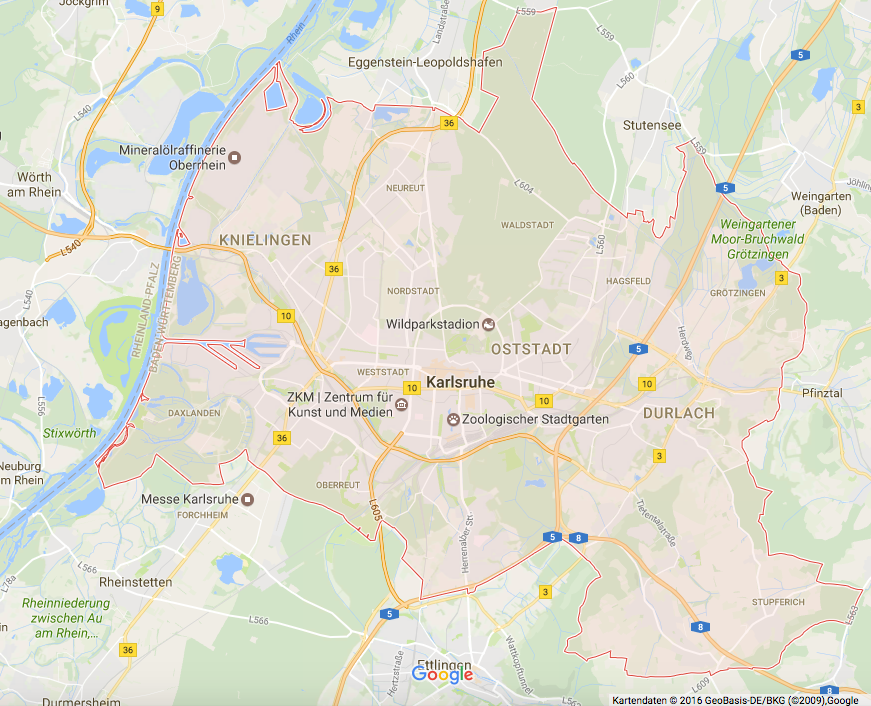
\includegraphics[width=0.55\textwidth]{Stadtgebiet_KA_zoom12.PNG}
    \caption{Darstellung der Gemarkungsgrenze des Stadtkreises Karlsruhe [Quelle: google maps, Zoomstufe 12]}
    \label{fig:Stadtgebiet_KA}
\end{figure}
%
Die Gemarkungsgrenze des Stadtkreises, wie sie in google maps bei einer Zoomstufe von \num{12} dargestellt wird, zeigt Abbildung \ref{fig:Stadtgebiet_KA}. Mit Hilfe des im vorliegenden Projekt entwickelten Verfahrens wird nun versucht, das Stadtgebiet durch die erzeugten Kacheln zu approximieren. Bei der Entscheidung, mit welcher Zoomstufe gearbeitet werden soll, gilt es, zwischen den Genauigkeitsanforderungen  der Daten und einer akzeptablen, zu verarbeitenden Datenmenge abzuwägen. 
%
\begin{figure}
  \centering
    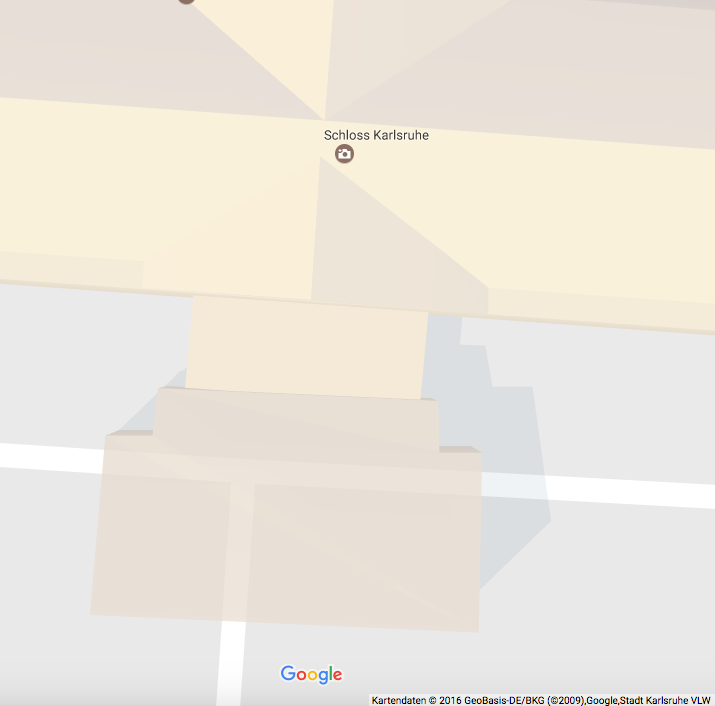
\includegraphics[width=0.4\textwidth]{KA_Schloss_zoom21.PNG}
    \caption{Darstellung des Karlsruher Schlosses bei höchster verfügbarer Zoomstufe [Quelle: google maps, Zoomstufe 21]}
    \label{fig:Schloss_KA}
\end{figure}
%
Stellt man das Karlsruher Stadtgebiet in google maps mit der maximale Zoomstufe von 21 wählbar, führt dies auf eine Darstellung auf Gebäudeebene, wie Abbildung \ref{fig:Schloss_KA} am Beispiel des Karlsruher Schlosses darstellt. Damit ist eine solche nicht geeignet, um das gesamte Stadtgebiet darzustellen, da entsprechend mehrere tausend Einzelkacheln erzeugt werden müssten. In der vorliegenden Kalibrierung wird mit einer (vergleichweise hohen) Zoomstufe von 17 gearbeitet. Diese liefert eine sehr hohe Auflösung des Gebietes und enthält alle zu untersuchenden Flächen in ausreichender Genauigkeit, gleichzeitig kann die Analyse mit noch akzeptablem Rechenaufwand durchgeführt werden. Allerdings ist hier bereits für das Stadtgebiet Karlsruhe eine sehr große Zahl an Einzelkacheln notwendig, weswegen für die spätere Anwendung eine geringere Zoomstufe empfohlen wird.\\
\newline
Da google maps die wählbaren Zoomstufen nicht mit einem festen kartographischen Maßstab verknüpft, muss dieser durch eigene Abstandsmessungen ermittelt werden. Bei Zoomstufe 17 besitzt eine der erzeugten quadratischen Einzelkacheln beispielsweise eine Kantenlänge von ca. \num{500} \si{\metre}.\\
%
\begin{figure}
  \centering
    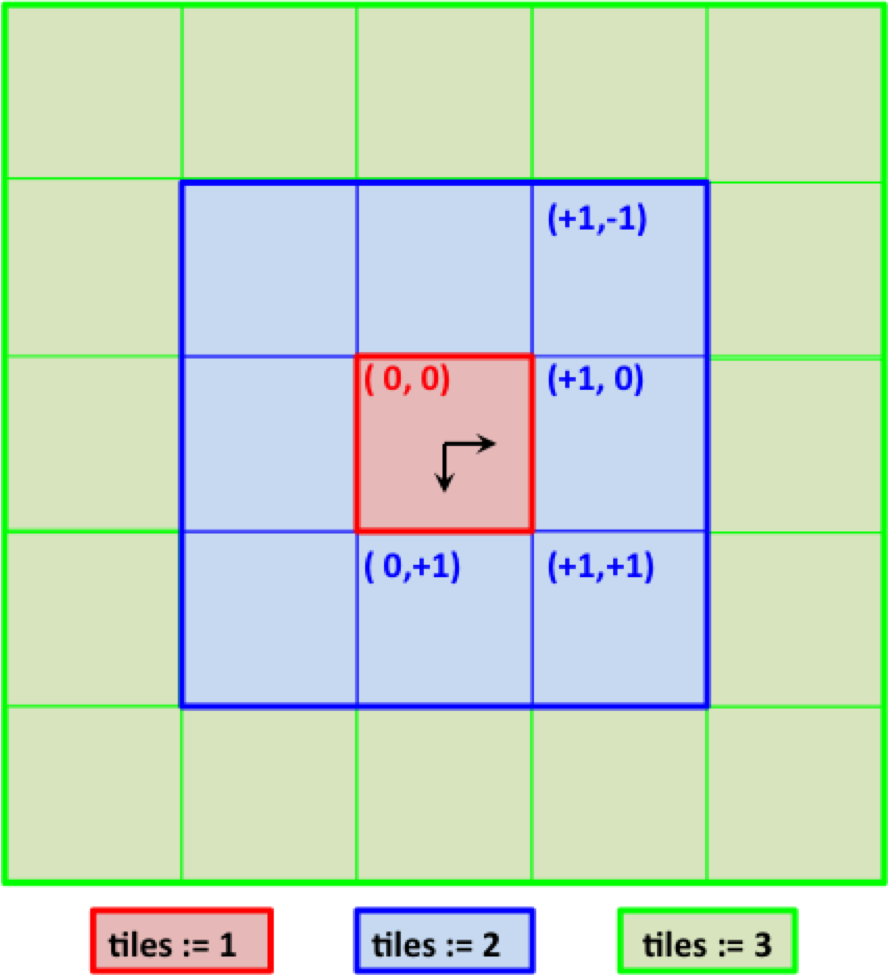
\includegraphics[width=0.4\textwidth]{Auswahl_tiles.png}
    \caption{Anordnung und Auswahl der Kacheln zur Städtebaulichen Analyse}
    \label{fig:Auswahl_tiles}
\end{figure}
%
Im Weiteren wird die Flächenanalyse nun für verschiedene Anzahlen an Kacheln durchgeführt. Das Prinzip der Kachelauswahl ist in Abbildung \ref{fig:Auswahl_tiles} dargestellt: eine Auswahl von \textit{n} tiles im Code erzeugt eine quadratische Analysefläche von \((2*n+1)^2\) Kacheln.\\
%
\newline
\begin{figure}
  \centering
    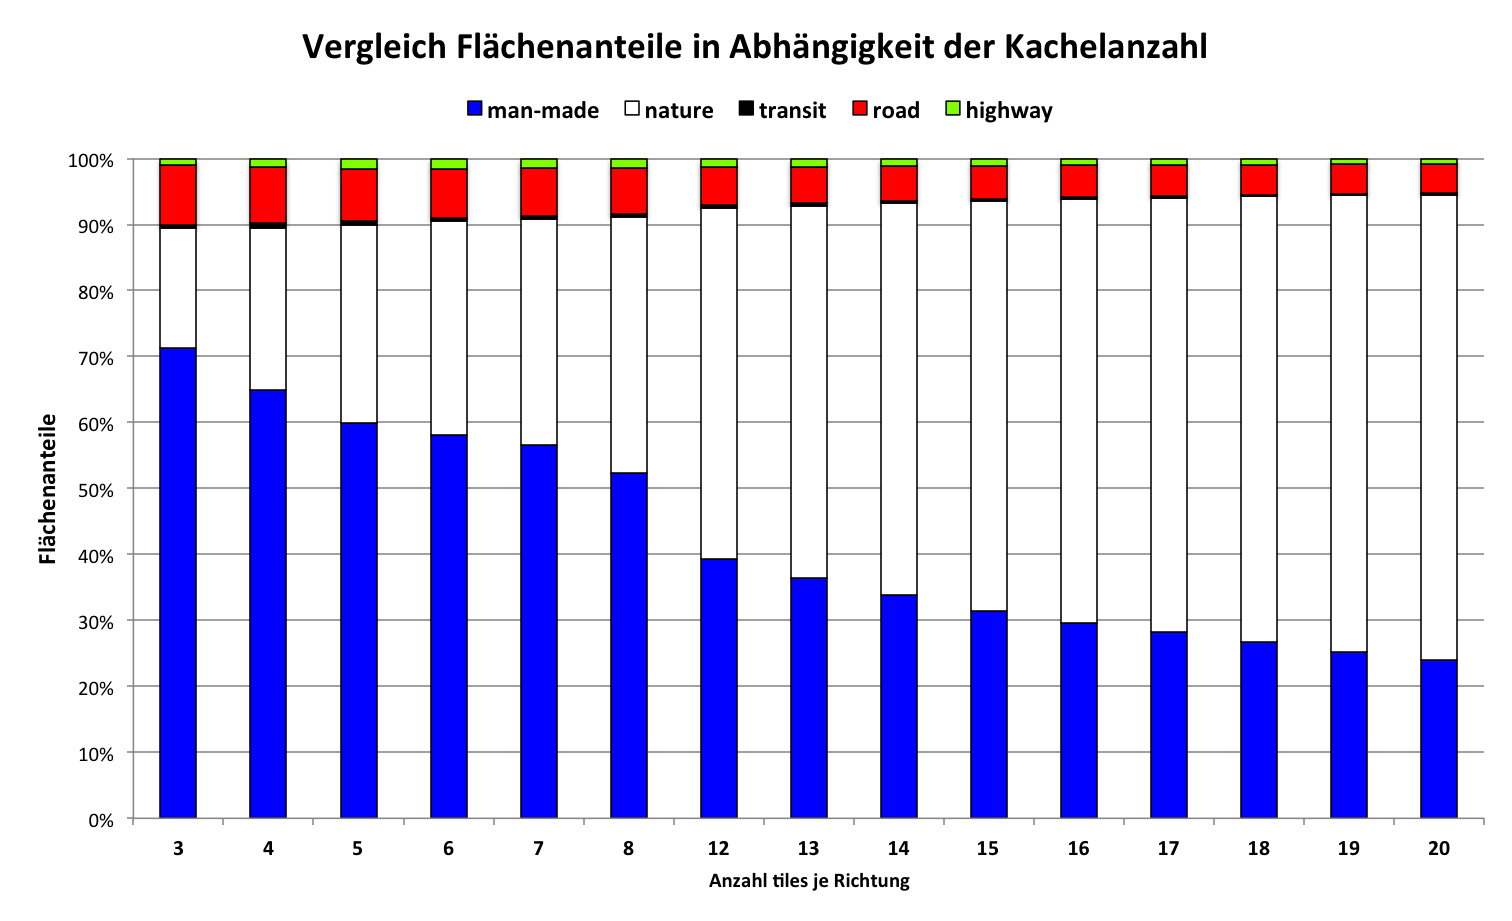
\includegraphics[width=0.85\textwidth]{Kachelvergleich_KA.png}
    \caption{Ergebnisse der Flächenanalyse für den Stadtkreis Karlsruhe für verschiedene Kachelanzahlen}
    \label{fig:Kachel_vgl}
\end{figure}
%
Die Ergebnisse einer Analyse der verschiedenen Nutzungsarten für das Karlsruher Stadtgebiet mit verschiedenen Kachelanzahlen sind in Abbildung \ref{fig:Kachel_vgl} dargestellt.\\
Die Auswahl weniger Kacheln ( \((n:=3)\) oder  \((n:=4)\)) führt auf kleine Analysequadrate mit Kantenlängen von \num{2.5} \si{\kilo\metre} bzw. \num{3.5} \si{\kilo\metre}, die nur das Zentrum der Stadt in die Analyse einbeziehen. Dementsprechend nimmt die man-made area mehr als \num{60} \% der Gesamtfläche ein, während die Naturfläche bei maximal \num{30} \% liegt.\\
Mit steigender Kachelzahl wird immer mehr des Stadtrandes und des Umlandes in die Analyse einbezogen, die Anteile von Verkehrsflächen und man-made area an der Gesamtfläche sinken deutlich ab zu Gunsten der Naturflächen, welche bei  \((n:=15)\) (Kantenlänge des Analysequadrates ca. \num{14.5} \si{\kilo\metre}) und  \((n:=16)\) (Kantenlänge des Analysequadrates ca. \num{15.5} \si{\kilo\metre}) mehr als \num{60} \% einnehmen. Die zuletzt erwähnten Kachelanzahlen erzeugen ein Analysequadrat, welches in seinen Ausdehnungen in der Größenordnung des Stadtgebiets liegt. Für eine vollkommene Umschließung des Stadtgebiets (maximale Nord-Süd-Ausdehnung ca. \num{16.5} \si{\kilo\metre}), maximale Ost-West-Ausdehnung ca. \num{19.0} \si{\kilo\metre}) muss für die Anzahl an Kacheln \((n:=20)\) gewählt werden.\\
Allerdings muss erwähnt werden, dass die in Abbildung \ref{fig:Stadtgebiet_KA} dargestellte Gemarkung durch eine solche quadratische Analysefläche nur unzureichend angenähert werden kann. In diesem Fall bedeutet es, dass bestimmte Bereiche wie beispielsweise große Teile des Ettlinger Stadtgebiets fälschlicherweise in der Analyse erscheinen. Eine bessere Approximation kann durch gezielte Auswahl bzw. gezieltes Ausschließen einzelner Kacheln erreicht werden.\\
Im Folgenden wird eine solche Auswahl vorgenommen, indem nur die entsprechenden Kacheln gewählt werden, die innerhalb des Karlsruher Stadtgebietes liegen.

Anhand des Beispiels Karlsruhe konnte damit gezeigt werden, dass das entwickelte Verfahren die reale Flächenverteilung gut annähern kann. 

% b) Verkehrliche Analyse
\newpage
\subsection{Verkehrsanalyse}

% c) Ableitung eines allgemeinen Leitfadens
\newpage
\subsection{Ableitung eines allgemeinen Leitfadens}

Um eine größere Menge verschiedener Städte möglichst schnell auf ihre verkehrliche Situation zu untersuchen, ist es sinnvoll, ein standardisiertes Vorgehen für die Erstellung einer Verkehrsuntersuchung festzulegen. Die Vorbereitung der Analyse läuft dabei wie folgt ab:

\begin{enumerate}
\item Die geographischen Koordinaten (lat, long) des Mittelpunktes der zentralen Kachel (0,0) wird festgelegt. Dies muss nicht zwingenderweise der in google oder bing maps hinterlegte zentrale Punkt einer Stadt sein. Vielmehr kann es durchaus sinnvoll sein, den Mittelpunkt möglichst mittig im später zu analysierenden Gebiet zu platzieren. Auf diese Weise kann die Anzahl benötigter Kacheln zur Abdeckung des Analysegebiets minimal gehalten werden.
\newline
\item Im Anschluss ist die Zoomstufe, in der die Kacheln geladen werden sollen, festzulegen. Hierbei treten zwei einschränkende Kriterien ein:\\
Einerseits wird in einigen Städten eine minimale Zoomstufe durch die Auflösung der Gebäude- und Flächendaten vorgegeben. Bei Unterschreitung dieser wird das Ergebnis dahingehend verfälscht, dass sehr detailliert dargestellte Gebäudeumrisse in einer zu niedrigen Zoomstufe nicht als man-made area erkannt werden, sondern vielmehr den Naturflächen zugerechnet werden.\\
Andererseits kann von Seiten der Verkehrsdaten eine minimale Zoomstufe notwendig sein, da kleinere Nebenstraßen z.T. erst in einer entsprechend hohen Zoomstufe angezeigt werden.\\
In jedem Fall ist bei der Wahl der Zoomstufe zwischen Auflösung der Daten sowie Rechen- bzw. Speicheraufwand abzuwägen. Um den Aufwand gering zu halten, sollte die minimal mögliche Zoomstufe nicht deutlich überschritten werden.
\newline
\item Anhand der gewählten Zoomstufe wird nun die Anzahl an benötigten Kacheln evaluiert, die notwendig ist, um das gesamte Untersuchungsgebiet abzudecken. 
\end{enumerate}


%%%%%%%%%%%%%
% 4) Fazit und Ausblick %
%%%%%%%%%%%%%
\newpage
\section{Fazit und Ausblick}



%%%%%%%%%%%%%%%%%%%%%%%%%%%%%%%
% Literaturverzeichnis (beginnt auf einer ungeraden Seite)   %
%%%%%%%%%%%%%%%%%%%%%%%%%%%%%%%
\newpage
\begin{thebibliography}{50}
\bibitem{advnutz} Arbeitsgemeinschaft der Vermessungsverwaltungen der Länder der Bundesrepublik Deutschland (AdV): \textit{Katalog der tatsächlichen Nutzungsarten im Liegenschaftskataster und ihrer Begriffsbestimmungen (AdV-Nutzungsartenkatalog)}, November 2011. Web. 29. Dez. 2016.\\ \url{http://www.adv-online.de/AdV-Produkte/Liegenschaftskataster/Download/binarywriterservlet?imgUid=3ea209e9-8835-5431-ce24-a4a2072e13d6&uBasVariant=11111111-1111-1111-1111-111111111111&isDownload=true}
\bibitem{StatBaWu_Flaeche} Statistisches Landesamt Baden-Württemberg: \textit{Statistische Berichte Baden-Württemberg - Flächenerhebung nach Art der tatsächlichen Nutzung 2015 - Stand 31.12.2015 -}, Juni 2016. Web. 29. Dez. 2016. \\ \url{http://www.statistik.baden-wuerttemberg.de/Service/Veroeff/Statistische_Berichte/333615001.pdf} 
\bibitem{StatBaWu_Einw} Statistisches Landesamt Baden-Württemberg: \textit{Statistische Berichte Baden-Württemberg - Bevölkerungsentwicklung in den Gemeinden Baden-Württembergs 2015}, Oktober 2016. Web. 29. Dez. 2016. \\ \url{http://www.statistik.baden-wuerttemberg.de/Service/Veroeff/Statistische_Berichte/312615001.pdf} 

	


 
\end{thebibliography}
 
      
  % ggf. hier Tabelle mit Symbolen 
  % (kann auch auf das Inhaltsverzeichnis folgen)

\newpage
  
 \thispagestyle{empty}


\vspace*{8cm}


\section*{Erklärung}

Hiermit versichere ich, dass ich diese Arbeit selbständig verfasst und keine anderen, als die angegebenen Quellen und Hilfsmittel benutzt, die wörtlich oder inhaltlich übernommenen Stellen als solche kenntlich gemacht und die Satzung des Karlsruher Instituts für Technologie zur Sicherung guter wissenschaftlicher Praxis in der jeweils gültigen Fassung beachtet habe. \\[2ex] 

\noindent
Ort, den Datum\\[5ex]

% Unterschrift (handgeschrieben)



\end{document}

